%!TEX root = ../cv.tex
% -*- root: ../cv.tex -*-

%-------------------------------------------------------------------------------
% SECTION TITLE
%-------------------------------------------------------------------------------
\cvsection{Experience}


%-------------------------------------------------------------------------------
% CONTENT
%-------------------------------------------------------------------------------
\begin{cventries}
%---------------------------------------------------------
  \cventry
    {Deep Learning} % Job title
    {} % Organization
    {} % Location
    {Level: B+} % Date(s)
    {
      \begin{cvitems} % Description(s) of tasks/responsibilities
        \item {결함 검출을 위한 딥러닝 기반 객체 검출(Object Detection) 알고리즘 연구}
        \item {차량 내 조향핸들 영역 분류(Classification) 기술 개발}
      \end{cvitems}
    }

%---------------------------------------------------------
  \cventry
    {Computer Vision and Pattern Recognition} % Job title
    {} % Organization
    {} % Location
    {Level: B+} % Date(s)
    {
      \begin{cvitems} % Description(s) of tasks/responsibilities
        \item {특징점 추적 기술 기반의 모바일 증강현실 기술 개발 \\
               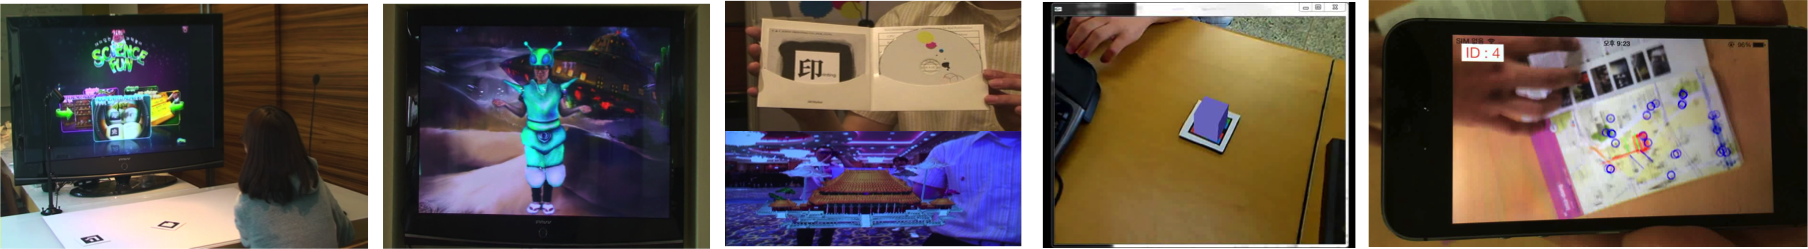
\includegraphics[width=\linewidth]{cv/resources/ar.png} }
          \begin{itemize}
            \item {인식 성능 및 속도 향상을 위한 특징점 Filtering기반 가속 특징점 매칭 기법 연구}
          \end{itemize}
        \item {깊이 인식 카메라 기반 손 인식 기술 개발 \\
               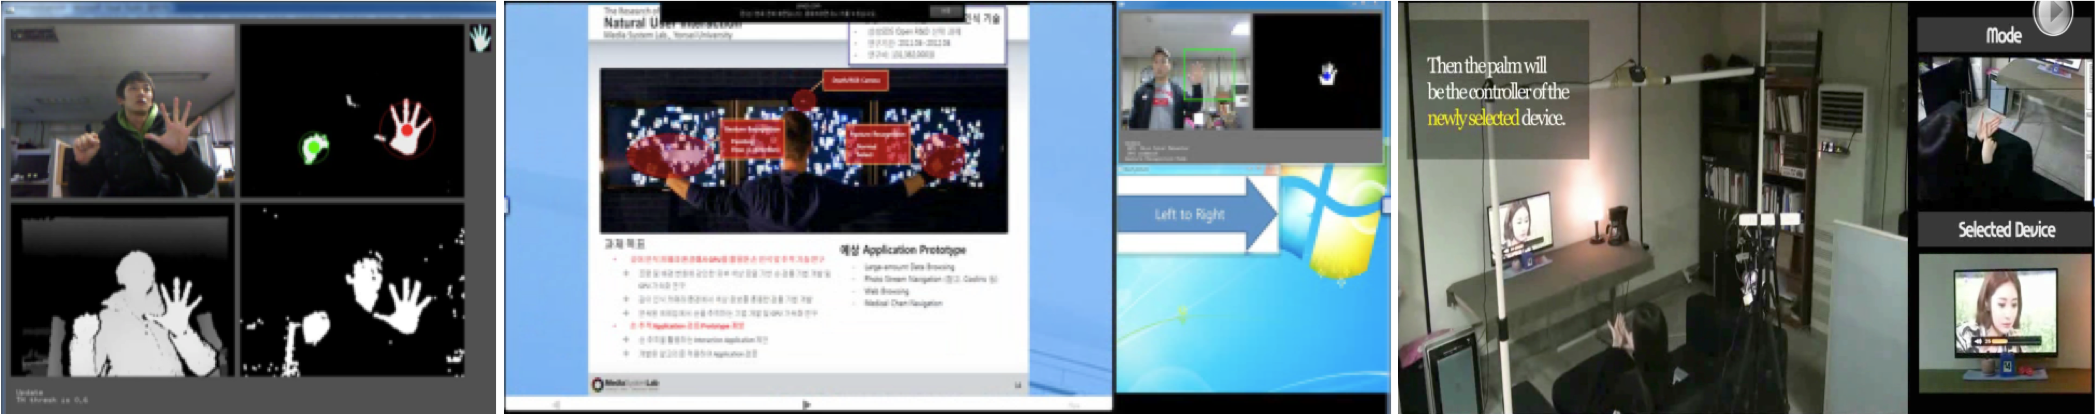
\includegraphics[width=\linewidth]{cv/resources/hand.png} }
        \item {차량 내 조향핸들 및 Spoke 영역 Tracking 기술 개발}
      \end{cvitems}
    }

%---------------------------------------------------------
  \cventry
    {Device Fast Prototyping} % Job title
    {} % Organization
    {} % Location
    {Level: A+} % Date(s)
    {
      \begin{cvitems} % Description(s) of tasks/responsibilities
        \item {$360^{\circ}$ 회전가능한 프로젝터를 이용한 퍼베이시브 컴퓨팅 환경 개발 \\
          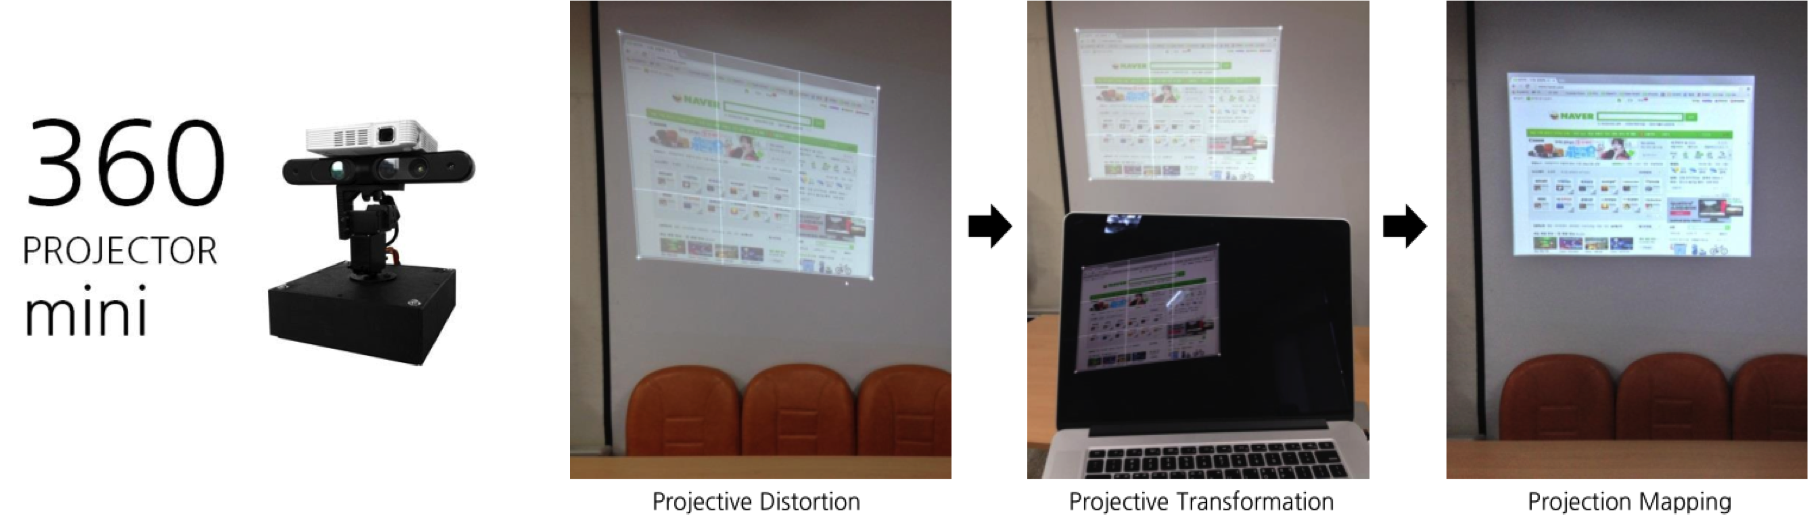
\includegraphics[width=\linewidth]{cv/resources/pervasiveAR.png}
          \begin{itemize}
              \item {피코 프로젝터, 소형 깊이 인식 카메라, Arduino 기반 Pan-Tilt 모터 시스템}
              \item {정규Pan-Tilt 에 따른 프로젝션 정규화 기술 개발 및 터치 기반 상호작용 기술 개발}
          \end{itemize}
        }
        \item {정보 증강이 가능한 펜 형태의 인터페이스 \\
          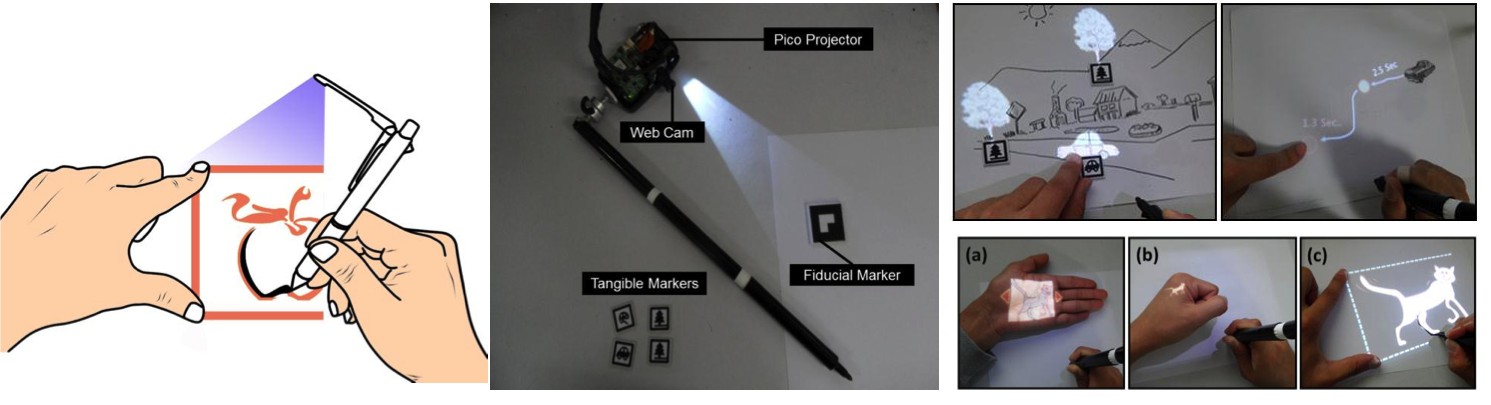
\includegraphics[width=\linewidth, height=40mm]{cv/resources/augpen.png}
          \begin{itemize}
            \item {피코 프로젝터, 소형 웹캠, Fiducial 마커}
            \item {2D 컨텐츠 및 손 인식 상호작용 기술 개발}
          \end{itemize}
        }
        \item {센서 기반 제스처 인터페이스 \\
          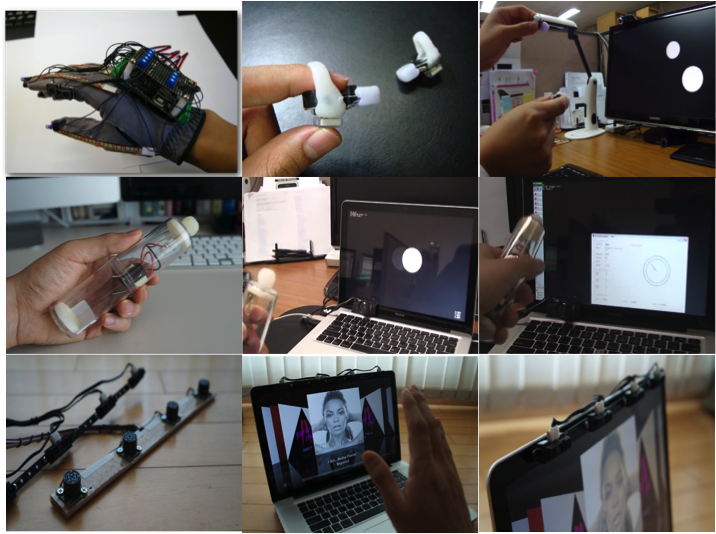
\includegraphics[width=\linewidth]{cv/resources/gesturedevices.png}
          \begin{itemize}
            \item {다양한 형태의 제스처 인식을 위한 센서 기기 개발}
            \item {IR Blob, Flex 센서, Gyro 센서, Lidar 센서 이용하여 다양한 형태의 인터페이스 제작}
          \end{itemize}
        }
      \end{cvitems} 
    }

\end{cventries}
